\clearpage

\section*{二、实验操作与原始数据}

\subsection*{1. 实际实验标准与测量顺序}

一切操作和数据处理按照上课课件标准处理。上文完整保留课前预习报告，作为预习记录；其中的六次自动测量计划和逐差法来自预习讲义，与上课要求不同，不作为本次实际测量次数和正式数据处理方法。

课堂要求完成一组自动七峰记录及一次完整的手动电压—电流测量，绘制手动曲线判定峰位，再对自动、手动两组峰位分别作线性拟合，报告激发电势、相关系数、斜率标准不确定度和相对误差。

本次我在手动测量之前、之后各进行了一次自动测量，因此实际顺序为“自动前测—手动测量—自动后测”。因为手动测量耗时较长，期间装置的热状态会发生漂移，因此有必要保留前后两组自动记录作对照。

\subsection*{2. 仪器参数与操作记录}

本台实验仪给出的三项电压参数及电流挡位如下：

\begin{center}
\begin{minipage}{\linewidth}
\centering

{\small
\setlength{\tabcolsep}{6pt}
\renewcommand{\arraystretch}{1.15}
\begin{tabular}{cc}
\toprule

项目 & 本次记录 \\

\midrule

灯丝电压 $U_{F_1F_2}$ & $3.44\ \mathrm V$ \\

第一栅压 $U_{G_1K}$ & $0.85\ \mathrm V$ \\

拒斥电压 $U_{G_2A}$ & $1.79\ \mathrm V$ \\

微电流测量挡位 & $\times10^{-9}\ \mathrm A$，电流记为 nA \\

手动加速电压范围与步长 & $0.5\text{--}100.0\ \mathrm V$，每步 $0.5\ \mathrm V$ \\

\bottomrule

\end{tabular}
}

\end{minipage}
\end{center}

首先完成接线、预热和微电流调零，按本台参数设置各电压，观察波形并调整显示，使峰谷能分辨。通电和调节过程中注意电压极性及实验管保护，避免电流突然剧增或微电流放大器过载。

第一次自动测量在手动测量前进行。切换实验仪到自动方式并启动扫描，观察示波器波形；测量结束后按峰序查询，把七个峰的加速电压和峰电流逐一记录。

\begin{figure}[H]
\centering
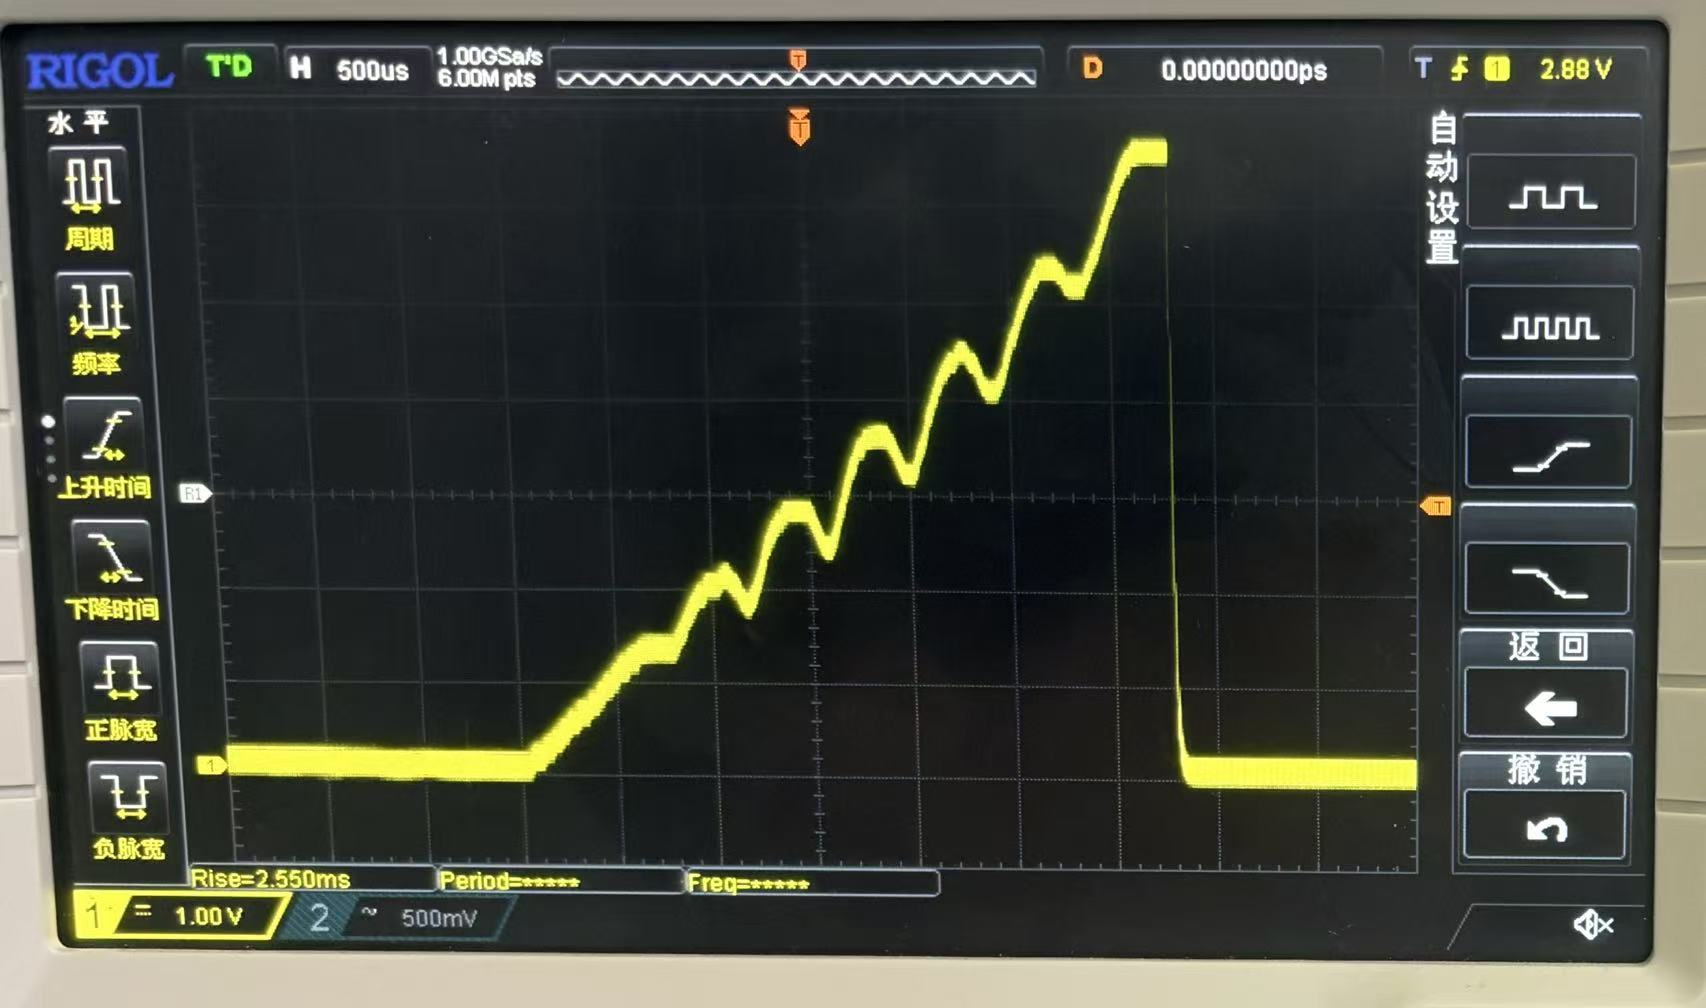
\includegraphics[width=\linewidth,height=.47\textheight,keepaspectratio]{../波形图.jpg}
\caption{本次自动扫描波形照片}
\end{figure}

随后切换到手动方式，从 0.5 V 起逐步增大加速电压，每隔 0.5 V 读取一组电压、电流，等待示数稳定后记录，直至 100.0 V，得到 200 个采样点。由于手动测量花费时间明显比一次自动扫描长，热电子发射和装置温度可能变化，不能把这 200 个点简单视为同一瞬间的扫描曲线。

手动测量结束后再次进行自动扫描，以相同的峰序记录七个峰位及峰电流，便于误差分析时考虑热漂移、读数稳定性及仪器工作状态的影响。

\subsection*{3. 原始记录与转录说明}

下图为本次原始数据。原表第 1 栏为“手动测量前”自动挡测得数据，第 3 栏为“手动测量后”自动挡测得数据。

\begin{figure}[H]
\centering
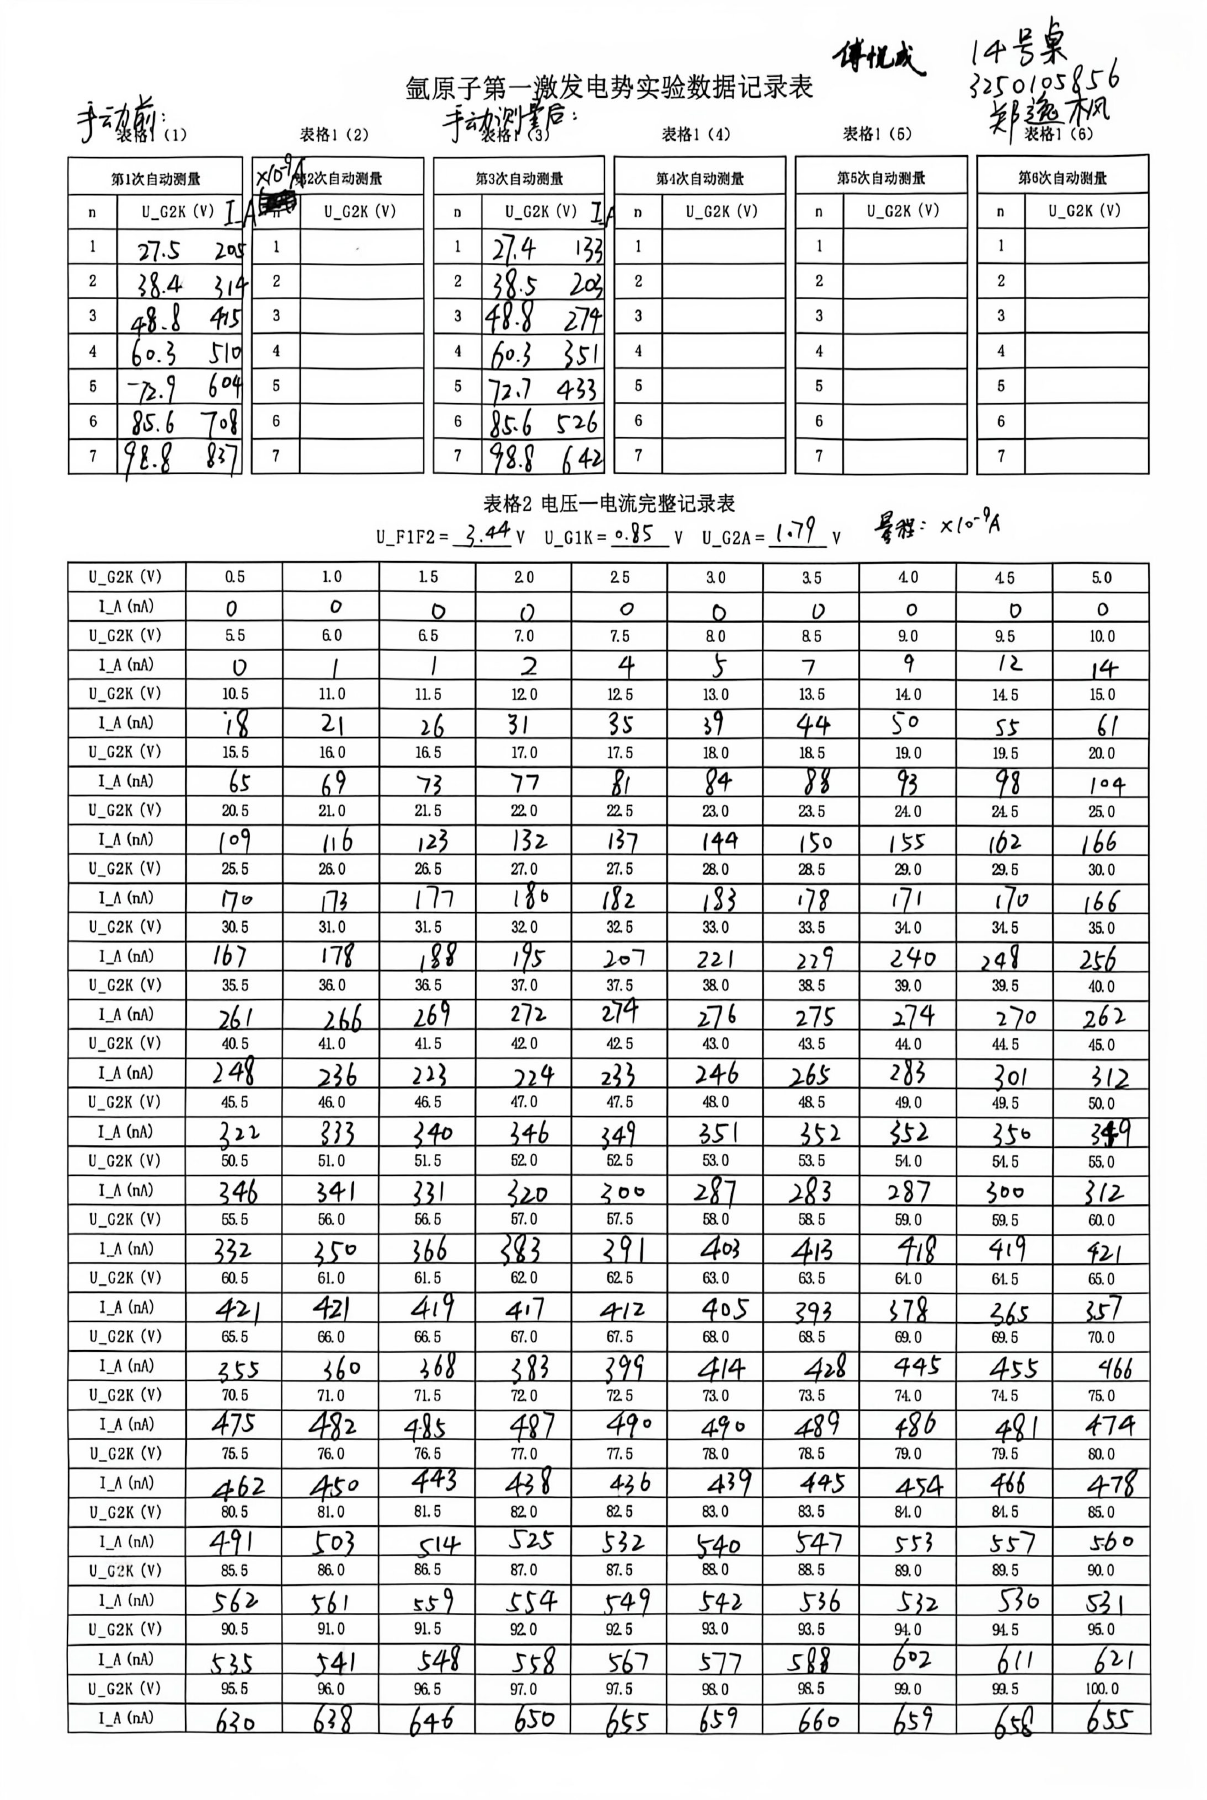
\includegraphics[height=14.5cm,keepaspectratio]{../assets/raw-data.png}
\caption{本次实验原始数据记录}
\end{figure}

\clearpage

\subsection*{4. 自动测量七峰记录}

\begin{center}
\begin{minipage}{\linewidth}
\centering

{\small
\setlength{\tabcolsep}{6pt}
\renewcommand{\arraystretch}{1.15}
\begin{tabular}{ccccc}
\toprule

峰序 $n$ & 前测峰位/V & 前测峰电流/nA & 后测峰位/V & 后测峰电流/nA \\

\midrule

1 & 27.5 & 205 & 27.4 & 133 \\

2 & 38.4 & 314 & 38.5 & 203 \\

3 & 48.8 & 415 & 48.8 & 274 \\

4 & 60.3 & 510 & 60.3 & 351 \\

5 & 72.9 & 604 & 72.7 & 433 \\

6 & 85.6 & 708 & 85.6 & 526 \\

7 & 98.8 & 837 & 98.8 & 642 \\

\bottomrule

\end{tabular}
}

\end{minipage}
\end{center}

\subsection*{5. 完整手动电压—电流记录}

\begingroup
\setstretch{1.1}

{\footnotesize
\setlength{\tabcolsep}{5pt}
\renewcommand{\arraystretch}{1.15}
\begin{longtable}{cccccccc}
\toprule

$U$/V & $I$/nA & $U$/V & $I$/nA & $U$/V & $I$/nA & $U$/V & $I$/nA \\

\midrule

\endfirsthead

\toprule

$U$/V & $I$/nA & $U$/V & $I$/nA & $U$/V & $I$/nA & $U$/V & $I$/nA \\

\midrule

\endhead

\bottomrule

\endfoot

0.5 & 0 & 25.5 & 170 & 50.5 & 346 & 75.5 & 462 \\

1.0 & 0 & 26.0 & 173 & 51.0 & 341 & 76.0 & 450 \\

1.5 & 0 & 26.5 & 177 & 51.5 & 331 & 76.5 & 443 \\

2.0 & 0 & 27.0 & 180 & 52.0 & 320 & 77.0 & 438 \\

2.5 & 0 & 27.5 & 182 & 52.5 & 300 & 77.5 & 436 \\

3.0 & 0 & 28.0 & 183 & 53.0 & 287 & 78.0 & 439 \\

3.5 & 0 & 28.5 & 178 & 53.5 & 283 & 78.5 & 445 \\

4.0 & 0 & 29.0 & 171 & 54.0 & 287 & 79.0 & 454 \\

4.5 & 0 & 29.5 & 170 & 54.5 & 300 & 79.5 & 466 \\

5.0 & 0 & 30.0 & 166 & 55.0 & 312 & 80.0 & 478 \\

5.5 & 0 & 30.5 & 167 & 55.5 & 332 & 80.5 & 491 \\

6.0 & 1 & 31.0 & 178 & 56.0 & 350 & 81.0 & 503 \\

6.5 & 1 & 31.5 & 188 & 56.5 & 366 & 81.5 & 514 \\

7.0 & 2 & 32.0 & 195 & 57.0 & 383 & 82.0 & 525 \\

7.5 & 4 & 32.5 & 207 & 57.5 & 391 & 82.5 & 532 \\

8.0 & 5 & 33.0 & 221 & 58.0 & 403 & 83.0 & 540 \\

8.5 & 7 & 33.5 & 229 & 58.5 & 413 & 83.5 & 547 \\

9.0 & 9 & 34.0 & 240 & 59.0 & 418 & 84.0 & 553 \\

9.5 & 12 & 34.5 & 248 & 59.5 & 419 & 84.5 & 557 \\

10.0 & 14 & 35.0 & 256 & 60.0 & 421 & 85.0 & 560 \\

10.5 & 18 & 35.5 & 261 & 60.5 & 421 & 85.5 & 562 \\

11.0 & 21 & 36.0 & 266 & 61.0 & 421 & 86.0 & 561 \\

11.5 & 26 & 36.5 & 269 & 61.5 & 419 & 86.5 & 559 \\

12.0 & 31 & 37.0 & 272 & 62.0 & 417 & 87.0 & 554 \\

12.5 & 35 & 37.5 & 274 & 62.5 & 412 & 87.5 & 549 \\

13.0 & 39 & 38.0 & 276 & 63.0 & 405 & 88.0 & 542 \\

13.5 & 44 & 38.5 & 275 & 63.5 & 393 & 88.5 & 536 \\

14.0 & 50 & 39.0 & 274 & 64.0 & 378 & 89.0 & 532 \\

14.5 & 55 & 39.5 & 270 & 64.5 & 365 & 89.5 & 530 \\

15.0 & 61 & 40.0 & 262 & 65.0 & 357 & 90.0 & 531 \\

15.5 & 65 & 40.5 & 248 & 65.5 & 355 & 90.5 & 535 \\

16.0 & 69 & 41.0 & 236 & 66.0 & 360 & 91.0 & 541 \\

16.5 & 73 & 41.5 & 223 & 66.5 & 368 & 91.5 & 548 \\

17.0 & 77 & 42.0 & 224 & 67.0 & 383 & 92.0 & 558 \\

17.5 & 81 & 42.5 & 233 & 67.5 & 399 & 92.5 & 567 \\

18.0 & 84 & 43.0 & 246 & 68.0 & 414 & 93.0 & 577 \\

18.5 & 88 & 43.5 & 265 & 68.5 & 428 & 93.5 & 588 \\

19.0 & 93 & 44.0 & 283 & 69.0 & 445 & 94.0 & 602 \\

19.5 & 98 & 44.5 & 301 & 69.5 & 455 & 94.5 & 611 \\

20.0 & 104 & 45.0 & 312 & 70.0 & 466 & 95.0 & 621 \\

20.5 & 109 & 45.5 & 322 & 70.5 & 475 & 95.5 & 630 \\

21.0 & 116 & 46.0 & 333 & 71.0 & 482 & 96.0 & 638 \\

21.5 & 123 & 46.5 & 340 & 71.5 & 485 & 96.5 & 646 \\

22.0 & 132 & 47.0 & 346 & 72.0 & 487 & 97.0 & 650 \\

22.5 & 137 & 47.5 & 349 & 72.5 & 490 & 97.5 & 665 \\

23.0 & 144 & 48.0 & 351 & 73.0 & 490 & 98.0 & 659 \\

23.5 & 150 & 48.5 & 352 & 73.5 & 489 & 98.5 & 660 \\

24.0 & 155 & 49.0 & 352 & 74.0 & 486 & 99.0 & 659 \\

24.5 & 162 & 49.5 & 350 & 74.5 & 481 & 99.5 & 656 \\

25.0 & 166 & 50.0 & 349 & 75.0 & 474 & 100.0 & 655 \\

\end{longtable}
}

\endgroup
